\section{Unit Testing}



\section{Test Driven Development}
With TDD, every feature 


At its core, TDD is made up of three iterative phases: "Red", "Green" and "Blue" (or "Refactor"):
\begin{itemize}
    \item In the "\textbf{Red}" phase, a test case is written for the chunk of functionality to be implemented; since the corresponding logic does not exist yet, the test will obviously fail, often not even compiling.
    \item In the "\textbf{Green}" phase, only the code that is strictly required to make the test pass is written.
    \item Finally, in the "\textbf{Blue}" phase, the implemented code, as well as the respective test cases, is refactored and improved. It is important to perform regression testing after the refactoring to ensure that the changes didn't result in any unexpected behaviors in other components.
\end{itemize}
Each new unit of code requires a repetition of this cycle \cite{GuidelinesTDD}.

The figure below provides a representation of the TDD cycle:
\begin{figure}[h]
    \centering
    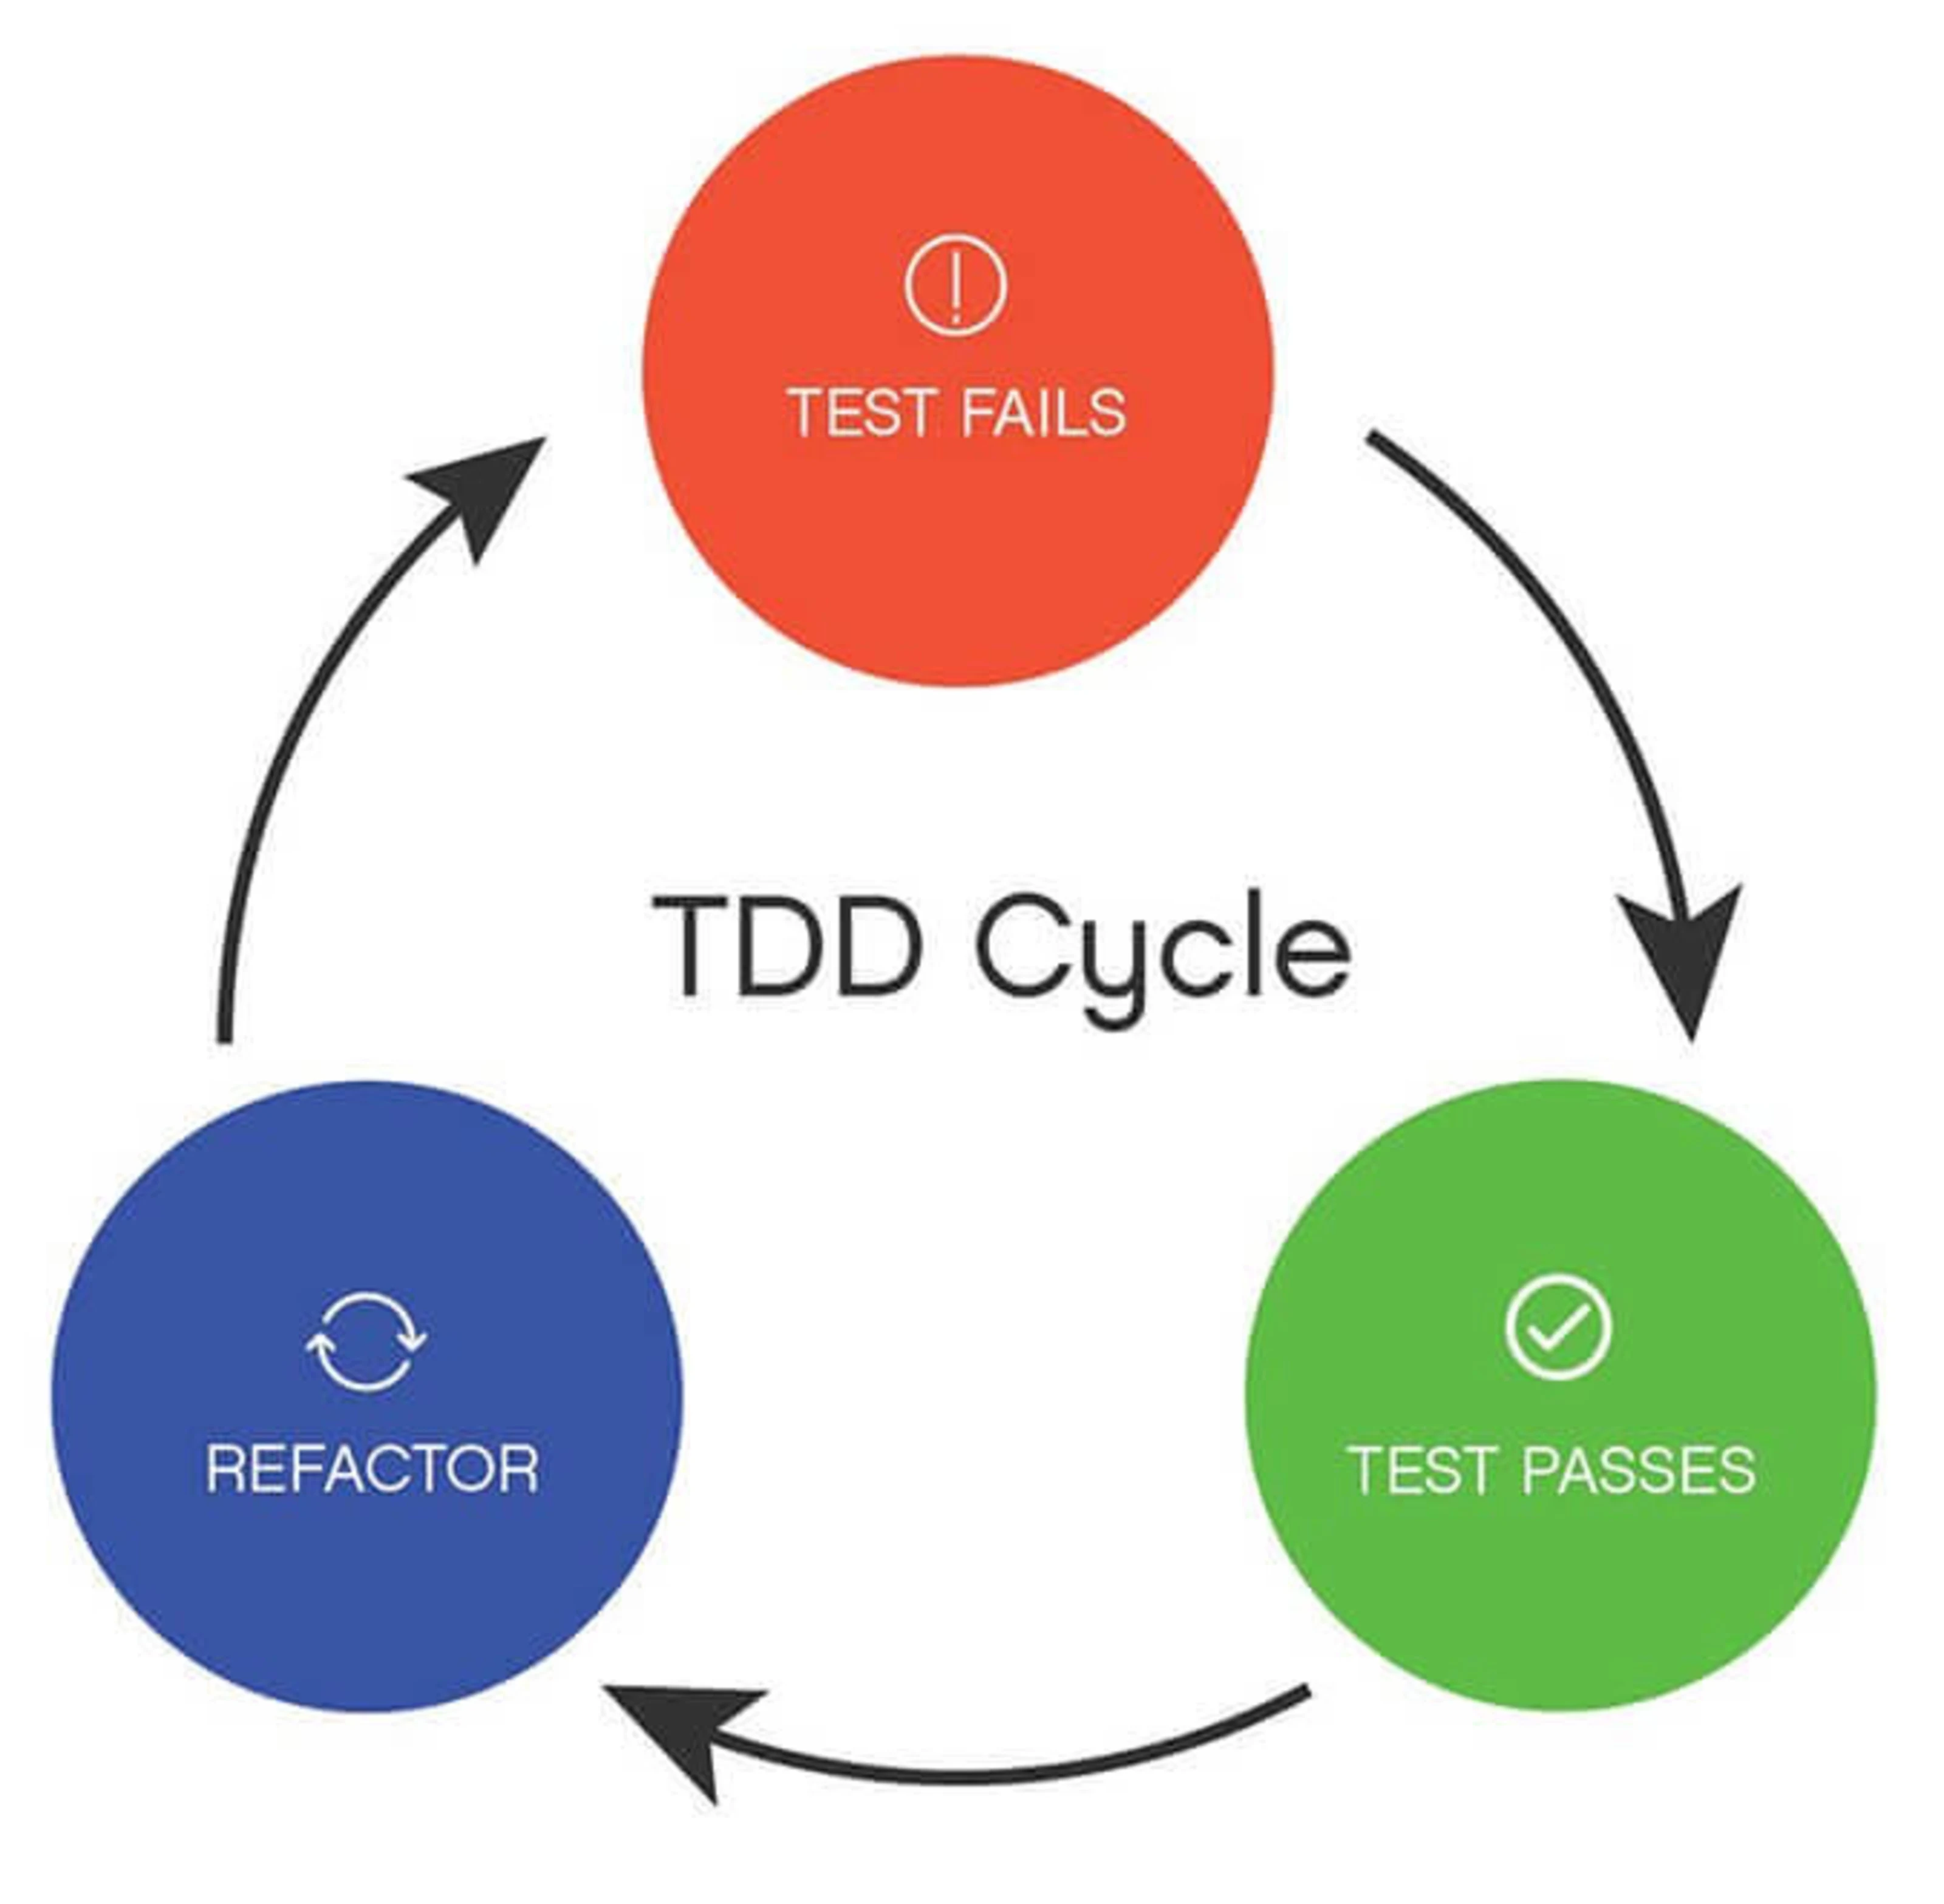
\includegraphics[width=\linewidth]{figures/tdd_cycle.jpg}
    \caption{The Test Driven Development cycle}
    \label{fig}
\end{figure}


The general mantra of TDD revolves around the "Make it green, then make it clean" motto


The employment of TDD can result in a series of benefits during the development process, sych as:
\begin{itemize}
    \item \textbf{Regression testing}: by incrementally building a test suite as the different iterations of TDD are performed, we ensure that the system  
    \item \textbf{Very high code coverage}: coverage is a metric used to determine how much of the code is being tested; it can be expressed according to different criteria such as statement coverage, i.e., how many statements in the code are reached by the test cases, branch coverage, i.e., how many conditional branches are executed during testing, or function coverage, i.e., how many functions are executed when running the test suite. While different coverage criteria result in different benefits, by employing TDD we ensure that any segment of code written has at least one associated test case.
    \item \textbf{Improved code quality}: as we are specifically writing code to pass the tests in place, and refactoring it after the "Green" phase, we ensure that the code is cleaner and overall more optimized, without any extra pieces of functionalities that may not be needed. 
    \item \textbf{Improved code readability and documentation}: test act as documentation...
    \item \item \textbf{Simplified debugging and early fault detection}: Whenever a test fails it becomes obvious which component has caused the fault: by adopting this incremental approach and performing regression testing, if a test fail we will be certain that the newly written code will be responsible. For this reason, faults are detected extremely early during the testing process, rather than potentially remaining hidden until the whole test suite has been built and executed.
\end{itemize}


\section{Testing Embedded Systems}
Embedded Systems (ES) can be defined as a combination of hardware components and software systems that seamlessly work together to achieve a specific purpose. Such systems can be dynamically programmed or have a fixed functionality set, and are often engineered to achieve a domain-specific, often critical, goal.
In recent years, such system have seen a surge in popularity, and have driven innovation forward in their respective areas of deployment: everywhere, spanning from the agricultural field, to the medical and energy ones, ES of various size and complexity are employed. \\
Due to their high specialization, ES often deal with time and resource constraints, both in hardware and in software; often these systems are battery-powered and therefore the hardware they are equipped with, often purpose built, must be highly efficient in its operations. Furthermore, from the software point-of-view, it is essential that the system operates deterministically and with real-time constrains. \\
Failures in ES should always be evident and identifiable quickly (a heart monitor should not fail quietly \cite{MakingEmbeddedSystems}). Given the high criticality of such systems, ensuring their dependability over the course of their lifespan is essential; ES can be deployed in extreme conditions (i.e., weather monitoring in extreme locations of the planet, devices inside the human body, or \dots), where maintenance operations cannot be performed regularly,  and high availability is expected. 




Furthermore, given the absence of a user interface in most cases, testing such systems can be particularly challenging, given the lack of immediate feedback.





\section{Test Driven Development for Embedded Systems}
Generally, the testing process of ES follows the X-in-the-loop paradigm \cite{DBLP:journals/software/GarousiFKY18}; subcategories in this area include model-in-the-loop, software-in-the-loop, processor-in-the-loop, hardware-in-the-loop, and system-in-the-loop.
Reference the old survey papers (i.e. X in the loop) that provide a summary of the main techniques